\documentclass[12pt]{article}

\usepackage[parfill]{parskip}
\usepackage{fancyhdr}
\usepackage[fleqn]{amsmath}
\usepackage{amssymb}
\usepackage{hyperref}
\usepackage{enumitem}
\usepackage{tikz}
\usetikzlibrary{arrows.meta}

\setcounter{MaxMatrixCols}{15}

\pagestyle{fancy}
\fancyhf{}
\setlength{\headheight}{15pt}
\lhead{\textbf{MAU22C00} Discrete Mathematics}
\rhead{Ted Johnson ‑ 19335618}
\rfoot{\thepage}

\newcommand{\qedsymbol}{\rule{0.7em}{0.7em}}
\def\<#1>{\langle\ignorespaces#1\unskip\rangle}

\urlstyle{same}
\hypersetup{colorlinks=true, linkcolor=blue, urlcolor=blue}

\usetikzlibrary{automata,positioning}
\tikzset{
	node distance=2cm,
	every path/.style = {thick},
	every node/.style = {thick, draw, circle, fill=gray!20}
}

\begin{document}

\section*{Assignment 4}

I have read and I understand the plagiarism provisions in the General Regulations of the University Calendar for the current year, found at \href{http://www.tcd.ie/calendar}{here}.
I have also completed the Online Tutorial on avoiding plagiarism ‘Ready Steady Write’, located \href{http://tcd-ie.libguides.com/plagiarism/ready-steady-write}{here}.

\subsection*{Exercise 1}

(30 points) Let $(V,E)$ be the graph with vertices $a$, $b$, $c$, $d$, $e$, $f$, $g$, $h$, $i$, $j$ and $k$, and edges $ab$, $bc$, $ac$, $cd$, $ch$, $de$, $eh$, $ef$, $eg$, $fg$, $hi$, $ij$, $hk$, $jk$ and $jh$.

\subsubsection*{Part (a)}

Draw this graph.

\subsubsection*{Solution}

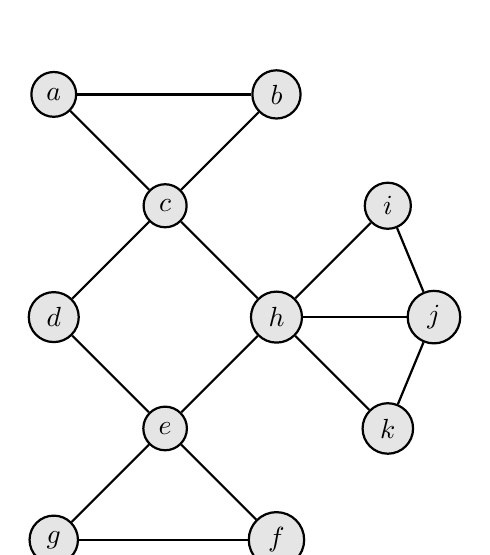
\begin{tikzpicture}
	\node (c) {$c$};
	\node (a) [above left of=c] {$a$};
	\node (b) [above right of=c] {$b$};
	\node (d) [below left of=c] {$d$};
	\node (e) [below right of=d] {$e$};
	\node (f) [below right of=e] {$f$};
	\node (g) [below left of=e] {$g$};
	\node (h) [below right of=c] {$h$};
	\node (i) [above right of=h] {$i$};
	\node (j) [right of=h] {$j$};
	\node (k) [below right of=h] {$k$};
	\draw (a) -- (b);
	\draw (a) -- (c);
	\draw (b) -- (c);
	\draw (c) -- (d);
	\draw (c) -- (h);
	\draw (d) -- (e);
	\draw (e) -- (h);
	\draw (e) -- (f);
	\draw (e) -- (g);
	\draw (f) -- (g);
	\draw (h) -- (i);
	\draw (h) -- (k);
	\draw (i) -- (j);
	\draw (j) -- (k);
	\draw (j) -- (h);
\end{tikzpicture}

\pagebreak
\subsubsection*{Part (b)}

Write down this graph's incidence table and its incidence matrix.

\subsubsection*{Solution}

Incidence table:

\begin{tabular}{c | *{15}{c}}
	& $ab$ & $bc$ & $ac$ & $cd$ & $ch$ & $de$ & $eh$ & $ef$ & $eg$ & $fg$ & $hi$ & $ij$ & $hk$ & $jk$ & $jh$ \\
	\hline
	$a$ & 1 & 0 & 1 & 0 & 0 & 0 & 0 & 0 & 0 & 0 & 0 & 0 & 0 & 0 & 0 \\
	$b$ & 1 & 1 & 0 & 0 & 0 & 0 & 0 & 0 & 0 & 0 & 0 & 0 & 0 & 0 & 0 \\
	$c$ & 0 & 1 & 1 & 1 & 1 & 0 & 0 & 0 & 0 & 0 & 0 & 0 & 0 & 0 & 0 \\
	$d$ & 0 & 0 & 0 & 1 & 0 & 1 & 0 & 0 & 0 & 0 & 0 & 0 & 0 & 0 & 0 \\
	$e$ & 0 & 0 & 0 & 0 & 0 & 1 & 1 & 1 & 1 & 0 & 0 & 0 & 0 & 0 & 0 \\
	$f$ & 0 & 0 & 0 & 0 & 0 & 0 & 0 & 1 & 0 & 1 & 0 & 0 & 0 & 0 & 0 \\
	$g$ & 0 & 0 & 0 & 0 & 0 & 0 & 0 & 0 & 1 & 1 & 0 & 0 & 0 & 0 & 0 \\
	$h$ & 0 & 0 & 0 & 0 & 1 & 0 & 1 & 0 & 0 & 0 & 1 & 0 & 1 & 0 & 1 \\
	$i$ & 0 & 0 & 0 & 0 & 0 & 0 & 0 & 0 & 0 & 0 & 1 & 1 & 0 & 0 & 0 \\
	$j$ & 0 & 0 & 0 & 0 & 0 & 0 & 0 & 0 & 0 & 0 & 0 & 1 & 0 & 1 & 1 \\
	$k$ & 0 & 0 & 0 & 0 & 0 & 0 & 0 & 0 & 0 & 0 & 0 & 0 & 1 & 1 & 0
\end{tabular}

\bigskip
Incidence matrix:
\[
\begin{pmatrix}
	1 & 0 & 1 & 0 & 0 & 0 & 0 & 0 & 0 & 0 & 0 & 0 & 0 & 0 & 0 \\
	1 & 1 & 0 & 0 & 0 & 0 & 0 & 0 & 0 & 0 & 0 & 0 & 0 & 0 & 0 \\
	0 & 1 & 1 & 1 & 1 & 0 & 0 & 0 & 0 & 0 & 0 & 0 & 0 & 0 & 0 \\
	0 & 0 & 0 & 1 & 0 & 1 & 0 & 0 & 0 & 0 & 0 & 0 & 0 & 0 & 0 \\
	0 & 0 & 0 & 0 & 0 & 1 & 1 & 1 & 1 & 0 & 0 & 0 & 0 & 0 & 0 \\
	0 & 0 & 0 & 0 & 0 & 0 & 0 & 1 & 0 & 1 & 0 & 0 & 0 & 0 & 0 \\
	0 & 0 & 0 & 0 & 0 & 0 & 0 & 0 & 1 & 1 & 0 & 0 & 0 & 0 & 0 \\
	0 & 0 & 0 & 0 & 1 & 0 & 1 & 0 & 0 & 0 & 1 & 0 & 1 & 0 & 1 \\
	0 & 0 & 0 & 0 & 0 & 0 & 0 & 0 & 0 & 0 & 1 & 1 & 0 & 0 & 0 \\
	0 & 0 & 0 & 0 & 0 & 0 & 0 & 0 & 0 & 0 & 0 & 1 & 0 & 1 & 1 \\
	0 & 0 & 0 & 0 & 0 & 0 & 0 & 0 & 0 & 0 & 0 & 0 & 1 & 1 & 0
\end{pmatrix}
\]

\pagebreak
\subsubsection*{Part (c)}

Write down this graph's adjacency table and its adjacency matrix.

\subsubsection*{Solution}

Adjacency table:

\begin{tabular}{c | *{11}{c}}
	& $a$ & $b$ & $c$ & $d$ & $e$ & $f$ & $g$ & $h$ & $i$ & $j$ & $k$ \\
	\hline
	$a$ & 0 & 1 & 1 & 0 & 0 & 0 & 0 & 0 & 0 & 0 & 0 \\
	$b$ & 1 & 0 & 1 & 0 & 0 & 0 & 0 & 0 & 0 & 0 & 0 \\
	$c$ & 1 & 1 & 0 & 1 & 0 & 0 & 0 & 1 & 0 & 0 & 0 \\
	$d$ & 0 & 0 & 1 & 0 & 1 & 0 & 0 & 0 & 0 & 0 & 0 \\
	$e$ & 0 & 0 & 0 & 1 & 0 & 1 & 1 & 1 & 0 & 0 & 0 \\
	$f$ & 0 & 0 & 0 & 0 & 1 & 0 & 1 & 0 & 0 & 0 & 0 \\
	$g$ & 0 & 0 & 0 & 0 & 1 & 1 & 0 & 0 & 0 & 0 & 0 \\
	$h$ & 0 & 0 & 1 & 0 & 1 & 0 & 0 & 0 & 1 & 1 & 1 \\
	$i$ & 0 & 0 & 0 & 0 & 0 & 0 & 0 & 1 & 0 & 1 & 0 \\
	$j$ & 0 & 0 & 0 & 0 & 0 & 0 & 0 & 1 & 1 & 0 & 1 \\
	$k$ & 0 & 0 & 0 & 0 & 0 & 0 & 0 & 1 & 0 & 1 & 0
\end{tabular}

\bigskip
Adjacency matrix:
\[
\begin{pmatrix}
	0 & 1 & 1 & 0 & 0 & 0 & 0 & 0 & 0 & 0 & 0 \\
	1 & 0 & 1 & 0 & 0 & 0 & 0 & 0 & 0 & 0 & 0 \\
	1 & 1 & 0 & 1 & 0 & 0 & 0 & 1 & 0 & 0 & 0 \\
	0 & 0 & 1 & 0 & 1 & 0 & 0 & 0 & 0 & 0 & 0 \\
	0 & 0 & 0 & 1 & 0 & 1 & 1 & 1 & 0 & 0 & 0 \\
	0 & 0 & 0 & 0 & 1 & 0 & 1 & 0 & 0 & 0 & 0 \\
	0 & 0 & 0 & 0 & 1 & 1 & 0 & 0 & 0 & 0 & 0 \\
	0 & 0 & 1 & 0 & 1 & 0 & 0 & 0 & 1 & 1 & 1 \\
	0 & 0 & 0 & 0 & 0 & 0 & 0 & 1 & 0 & 1 & 0 \\
	0 & 0 & 0 & 0 & 0 & 0 & 0 & 1 & 1 & 0 & 1 \\
	0 & 0 & 0 & 0 & 0 & 0 & 0 & 1 & 0 & 1 & 0
\end{pmatrix}
\]

\pagebreak
\subsubsection*{Part (d)}

Is this graph complete? Justify your answer.

\subsubsection*{Solution}

The graph is not complete. For example, edge $ad \notin E$, therefore $(V, E)$ is not complete.

\subsubsection*{Part (e)}

Is this graph bipartite? Justify your answer.

\subsubsection*{Solution}

The graph is not bipartite. The graph contains the complete subgraph $(V', E')$ where $V' = \{ a, b, c \}$ and $E' = \{ ab, ac, bc \}$ which cannot be partitioned.

\subsubsection*{Part (f)}

Is this graph regular? Justify your answer.

\subsubsection*{Solution}

The graph is not regular. For example, vertex $a$ has a degree of 2 while vertex $h$ has a degree of 5.

\subsubsection*{Part (g)}

Does this graph have any regular subgraph? Justify your answer.

\subsubsection*{Solution}

The graph does have a regular subgraph. For example, the subgraph $(V', E')$ where $V' = \{ a, b \}$ and $E' = \{ ab \}$ is 1-regular.

\pagebreak
\subsubsection*{Part (h)}

Give an example of an isomorphism $\varphi$ from the graph $(V,E)$ to itself satisfying that $\varphi(i) = k$.

\subsubsection*{Solution}

A possible isomorphism $\varphi$:\\
$\varphi(a) = a$, $\varphi(b) = b$, $\varphi(c) = c$, $\varphi(d) = d$, $\varphi(e) = e$, $\varphi(f) = f$,
$\varphi(g) = g$, $\varphi(h) = h$, $\varphi(i) = k$, $\varphi(j) = j$, $\varphi(k) = i$.

\subsubsection*{Part (i)}

Is the isomorphism from part (h) unique or can you find another isomorphism $\Psi$ that is distinct from $\varphi$ but also satisfies that $\Psi(i) = k$? Justify your answer.

\subsubsection*{Solution}

Isomorphism $\varphi$ is not unique. Another distinct possible isomorphism $\Psi$:\\
$\Psi(a) = g$, $\Psi(b) = f$, $\Psi(c) = e$, $\Psi(d) = d$, $\Psi(e) = c$, $\Psi(f) = b$,
$\Psi(g) = a$, $\Psi(h) = h$, $\Psi(i) = i$, $\Psi(j) = j$, $\Psi(k) = k$.

\subsubsection*{Part (j)}

Is this graph connected? Justify your answer.

\subsubsection*{Solution}

The graph is connected as there is a walk from from every vertex to every other vertex in $V$ traversing edges in $E$.

\subsubsection*{Part (k)}

Does this graph have an Eulerian trail? Justify your answer.

\subsubsection*{Solution}

We can count that $\deg h$ and $\deg j$ are odd while the rest of the vertices have even degrees. Thus there are exactly two vertices with odd degrees.
$\therefore$ The graph must have an Eulerian trail as proven in lectures.

\pagebreak
\subsubsection*{Part (l)}

Does this graph have an Eulerian circuit? Justify your answer.

\subsubsection*{Solution}

The graph cannot have an Eulerian circuit as for an Eulerian circuit to exist, every vertex must have an even degree.
In this case, $\deg h = 5$, so the graph does not have an Eulerian circuit.

\subsubsection*{Part (m)}

Does this graph have a Hamiltonian circuit? Justify your answer.

\subsubsection*{Solution}

It is impossible for the graph to have a Hamiltonian circuit as any must pass through vertex $h$ twice, disqualifying the circuit.

\subsubsection*{Part (n)}

Is this graph a tree? Justify your answer.

\subsubsection*{Solution}

The graph is not a tree as it contains a circuit. For example, $abc$ is a circuit.

\pagebreak
\subsection*{Exercise 2}

(10 points) Prove that a connected graph $(V,E)$ is a tree if and only if adding an edge between any two vertices in $(V,E)$ creates exactly one circuit.

\subsubsection*{Solution}

We will prove this equivalence relation by proving each direction separately:

'$\implies$' Assuming a connected graph $(V,E)$ is a tree, prove adding an edge between any two vertices in $(V,E)$ creates exactly one circuit.
\begin{quote}
	As proven in lectures, $\forall v,w \in V$ where $v \ne w$ it can be shown that there exists exactly one distinct path in the tree $(V,E)$ from $v$ to $w$.
	Given that $v$ and $w$ are not already adjacent, by adding the edge $vw$ to $(V,E)$, we have created a second distinct path between $v$ and $w$.
	In other words, there are now exactly two distinct paths between $v$ and $w$. As proven in lectures, this implies the graph now contains at least one simple circuit.

	However, we can confirm that exactly one circuit has been created.
	If two distinct circuits were formed by the addition of edge $vw$, the removal of edge $vw$ would leave two distinct paths from $v$ to $w$.
	This is a contradiction as tree $(V,E)$ may not have two distinct paths from two vertices.
	Thus the addition of edge $vw$ to tree $(V,E)$ creates exactly one circuit.
\end{quote}

'$\impliedby$' Assuming adding an edge between any two vertices in a connected graph $(V,E)$ creates exactly one circuit, prove $(V,E)$ is a tree.
\begin{quote}
	If adding an edge to the connected graph $(V,E)$ creates exactly one circuit, then prior to the addition of the edge the graph $(V,E)$ must have no circuits.
	That is, the graph $(V,E)$ would be an acyclic connected graph. Notice that this is exactly the definition of a tree, therefore the statement holds.
\end{quote}

Both directions of the equivalence relation have been proven so the relation must hold.
\\\null\hfill\qedsymbol

\pagebreak
\subsection*{Exercise 3}

Consider the connected graph with vertices $A$, $B$, $C$, $D$, $E$, $F$, $G$, $H$, $I$, $J$, $K$ and $L$,
and with edges, listed with associated costs, in the following table:

\begin{tabular}{*{12}{c}}
	FJ & JK & CH & EI & DJ & AB & EH & FK & BG & GJ & BC & AF \\
	1  & 1  & 1  & 1  & 2  & 2  & 2  & 2  & 3  & 3  & 3  & 3 \\
	AC & EF & DF & DL & HI & CE & BD & AD & AE & GL & EK & JL \\
	3  & 4  & 4  & 4  & 5  & 6  & 6  & 6  & 6  & 7  & 7  & 8
\end{tabular}

\subsubsection*{Part (a)}

(2 points) Draw the graph and label each edge with its cost.

\subsubsection*{Solution}

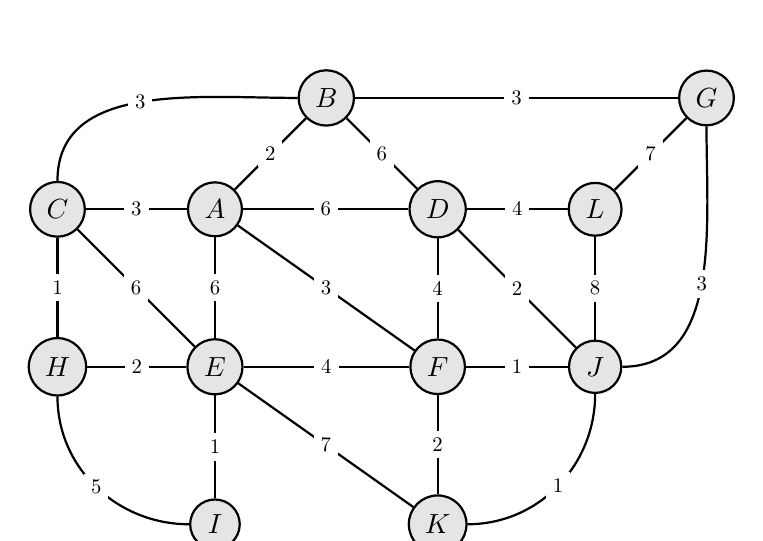
\begin{tikzpicture}[weight/.style={draw=none,rectangle,scale=0.75,fill=white}]
	\node (b) {$B$};
	\node (a) [below left of=b] {$A$};
	\node (d) [below right of=b] {$D$};
	\node (c) [left of=a] {$C$};
	\node (l) [right of=d] {$L$};
	\node (g) [above right of=l] {$G$};
	\node (j) [below of=l] {$J$};
	\node (f) [below of=d] {$F$};
	\node (e) [below of=a] {$E$};
	\node (h) [below of=c] {$H$};
	\node (k) [below of=f] {$K$};
	\node (i) [below of=e] {$I$};
	\draw (f) -- node [weight] {1} (j);
	\draw (j) to [out=270,in=0,looseness=1] node [weight] {1} (k);
	\draw (c) -- node [weight] {1} (h);
	\draw (e) -- node [weight] {1} (i);
	\draw (d) -- node [weight] {2} (j);
	\draw (a) -- node [weight] {2} (b);
	\draw (e) -- node [weight] {2} (h);
	\draw (f) -- node [weight] {2} (k);
	\draw (b) -- node [weight] {3} (g);
	\draw (g) to [out=270,in=0,looseness=1] node [weight] {3} (j);
	\draw (b) to [out=180,in=90,looseness=1] node [weight] {3} (c);
	\draw (a) -- node [weight] {3} (f);
	\draw (a) -- node [weight] {3} (c);
	\draw (e) -- node [weight] {4} (f);
	\draw (f) -- node [weight] {4} (d);
	\draw (d) -- node [weight] {4} (l);
	\draw (h) to [out=270,in=180,looseness=1] node [weight] {5} (i);
	\draw (c) -- node [weight] {6} (e);
	\draw (b) -- node [weight] {6} (d);
	\draw (a) -- node [weight] {6} (d);
	\draw (a) -- node [weight] {6} (e);
	\draw (g) -- node [weight] {7} (l);
	\draw (e) -- node [weight] {7} (k);
	\draw (j) -- node [weight] {8} (l);
\end{tikzpicture}

\pagebreak
\subsubsection*{Part (b)}

(9 points) Determine the minimum spanning tree generated by Kruskal's Algorithm, where that algorithm is applied with the queue specified in the table above.
For each step of the algorithm, write down the edge that is added.

\subsubsection*{Solution}

We start with $(V, \emptyset)$, the subgraph of the graph consisting of all the vertices and none of the edges.
We then add edges to this subgraph in the following order:
$\{ FJ, JK, CH, EI, DJ, AB, EH, BG, GJ, AC, DL \}$
This generates the following minimum spanning tree:

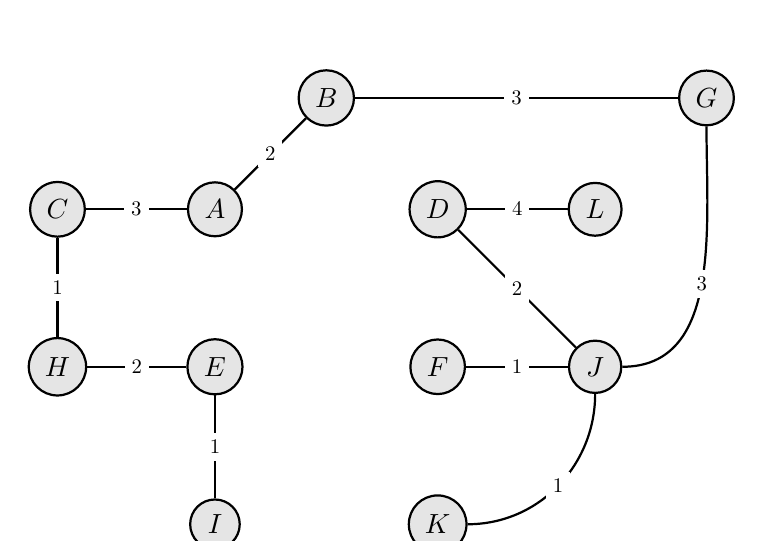
\begin{tikzpicture}[weight/.style={draw=none,rectangle,scale=0.75,fill=white}]
	\node (b) {$B$};
	\node (a) [below left of=b] {$A$};
	\node (d) [below right of=b] {$D$};
	\node (c) [left of=a] {$C$};
	\node (l) [right of=d] {$L$};
	\node (g) [above right of=l] {$G$};
	\node (j) [below of=l] {$J$};
	\node (f) [below of=d] {$F$};
	\node (e) [below of=a] {$E$};
	\node (h) [below of=c] {$H$};
	\node (k) [below of=f] {$K$};
	\node (i) [below of=e] {$I$};
	\draw (f) -- node [weight] {1} (j);
	\draw (j) to [out=270,in=0,looseness=1] node [weight] {1} (k);
	\draw (c) -- node [weight] {1} (h);
	\draw (e) -- node [weight] {1} (i);
	\draw (d) -- node [weight] {2} (j);
	\draw (a) -- node [weight] {2} (b);
	\draw (e) -- node [weight] {2} (h);
	\draw (b) -- node [weight] {3} (g);
	\draw (g) to [out=270,in=0,looseness=1] node [weight] {3} (j);
	\draw (a) -- node [weight] {3} (c);
	\draw (d) -- node [weight] {4} (l);
\end{tikzpicture}

\pagebreak
\subsubsection*{Part (c)}

(9 points) Determine the minimum spanning tree generated by Prim's Algorithm, starting from the vertex $D$, where that algorithm is applied with the queue specified in the table above.
For each step of the algorithm, write down the edge that is added.

\subsubsection*{Solution}

We start with $(\{ D \}, \emptyset)$, the subgraph of the graph consisting of the single vertex $D$ and none of the edges.
We then add the edges and its incident vertex that is not already included in the subgraph to the subgraph in the following order:
$\{ DJ, FJ, JK, GJ, BG, BA, BC, CH, EH, EI, DL \}$
This generates the following minimum spanning tree:

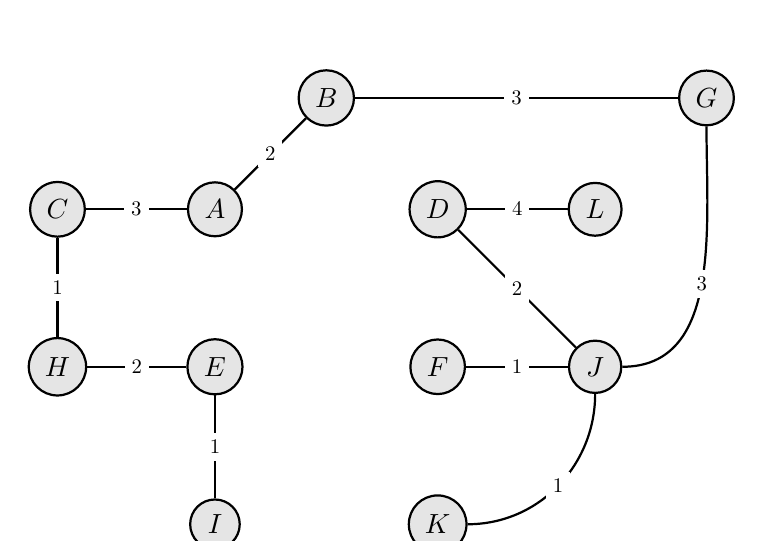
\begin{tikzpicture}[weight/.style={draw=none,rectangle,scale=0.75,fill=white}]
	\node (b) {$B$};
	\node (a) [below left of=b] {$A$};
	\node (d) [below right of=b] {$D$};
	\node (c) [left of=a] {$C$};
	\node (l) [right of=d] {$L$};
	\node (g) [above right of=l] {$G$};
	\node (j) [below of=l] {$J$};
	\node (f) [below of=d] {$F$};
	\node (e) [below of=a] {$E$};
	\node (h) [below of=c] {$H$};
	\node (k) [below of=f] {$K$};
	\node (i) [below of=e] {$I$};
	\draw (f) -- node [weight] {1} (j);
	\draw (j) to [out=270,in=0,looseness=1] node [weight] {1} (k);
	\draw (c) -- node [weight] {1} (h);
	\draw (e) -- node [weight] {1} (i);
	\draw (d) -- node [weight] {2} (j);
	\draw (a) -- node [weight] {2} (b);
	\draw (e) -- node [weight] {2} (h);
	\draw (b) -- node [weight] {3} (g);
	\draw (g) to [out=270,in=0,looseness=1] node [weight] {3} (j);
	\draw (a) -- node [weight] {3} (c);
	\draw (d) -- node [weight] {4} (l);
\end{tikzpicture}

\pagebreak
\subsection*{Exercise 4}

(10 points) Let $(V,E)$ be the directed graph with vertices $A$, $B$, $C$, $D$ and $E$, and edges $(A,A)$, $(C,A)$, $(A,B)$, $(B,C)$, $(D,C)$, $(C,E)$, $(E,E)$ and $(E,D)$.

\subsubsection*{Part (a)}

Draw this graph.

\subsubsection*{Solution}

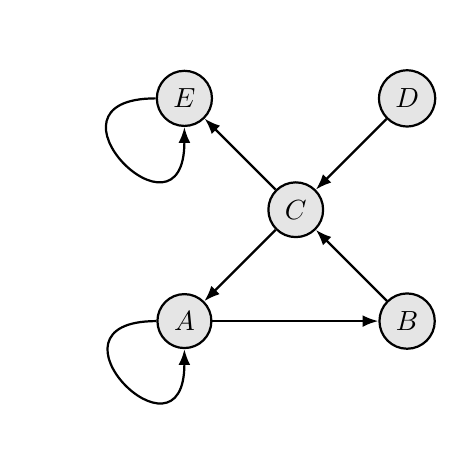
\begin{tikzpicture}[-{Latex[length=2mm]}]
	\node (c) {$C$};
	\node (a) [below left of=c] {$A$};
	\node (b) [below right of=c] {$B$};
	\node (d) [above right of=c] {$D$};
	\node (e) [above left of=c] {$E$};
	\draw (d) -- (c);
	\draw (c) -- (a);
	\draw (c) -- (e);
	\draw (a) to [out=180,in=270,looseness=8] (a);
	\draw (a) -- (b);
	\draw (b) -- (c);
	\draw (e) to [out=180,in=270,looseness=8] (e);
\end{tikzpicture}

\subsubsection*{Part (b)}

Write down this graph's adjacency matrix.

\subsubsection*{Solution}

Adjacency matrix, in the order $\{ A, B, C, D, E \}$:
\[
\begin{pmatrix}
	1 & 1 & 0 & 0 & 0 \\
	0 & 0 & 1 & 0 & 0 \\
	1 & 0 & 0 & 0 & 1 \\
	0 & 0 & 1 & 0 & 0 \\
	0 & 0 & 0 & 0 & 1
\end{pmatrix}
\]

\subsubsection*{Part (c)}

Give an example of an isomorphism $\varphi$ from the graph $(V,E)$ to itself such that $\varphi(A) = E$.
Note that an isomorphism of directed graphs should also respect the direction of the edges.

\subsubsection*{Solution}

$\varphi(A) = E$, $\varphi(B) = A$, $\varphi(C) = C$, $\varphi(D) = B$, $\varphi(E) = D$.

\pagebreak
\subsection*{Exercise 5}

(10 points) Let $R$ be a relation on a set $V = \{\,a,b,c,d,e,f\,\}$ given by $R = \{\,(a,c),(a,d),(c,c),(d,d),(b,b),(e,e),(b,e),(e,f),(f,e),(e,b),(f,f)\,\}$.

\subsubsection*{Part (a)}

Using the one-to-one correspondence between relations on finite sets and directed graphs, draw the directed graph corresponding to the relation $R$.

\subsubsection*{Solution}

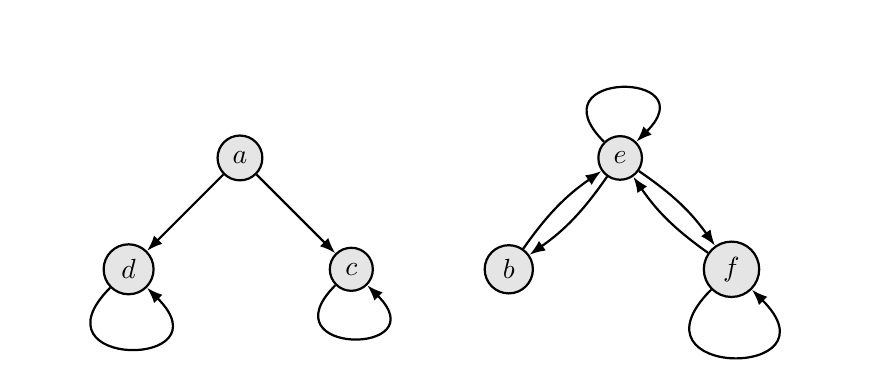
\begin{tikzpicture}[-{Latex[length=2mm]}]
	\node (d) {$d$};
	\node (a) [above right of=d] {$a$};
	\node (c) [below right of=a] {$c$};
	\node (b) [right of=c] {$b$};
	\node (e) [above right of=b] {$e$};
	\node (f) [below right of=e] {$f$};
	\draw (a) -- (c);
	\draw (a) -- (d);
	\draw (c) to [out=225,in=315,looseness=8] (c);
	\draw (d) to [out=225,in=315,looseness=8] (d);
	\draw (e) to [out=135,in=45,looseness=8] (e);
	\draw (b) to [bend left=10] (e);
	\draw (e) to [bend left=10] (f);
	\draw (f) to [bend left=10] (e);
	\draw (e) to [bend left=10] (b);
	\draw (f) to [out=225,in=315,looseness=8] (f);
\end{tikzpicture}

\subsubsection*{Part (b)}

Is $R$ an equivalence relation? Justify your answer.

\subsubsection*{Solution}

Relation $R$ is not an equivalence relation.
Relation $R$ is said to be an equivalence relation if and only if the relation is reflexive, symmetric and transitive.
However, it is clear from the directed graph that the relation $R$ does not exhibit any of these properties.

\begin{itemize}
	\item $(a,a) \notin R$. Therefore $R$ is not reflexive.
	\item $(a,d) \in R$ but $(d,a) \notin R$. Therefore $R$ is not symmetric.
	\item $(b,e),(e,f) \in R$ but $(b,f) \notin R$. Therefore $R$ is not transitive.
\end{itemize}

\subsubsection*{Part (c)}

If $R$ is not an equivalence relation, which ordered pairs would have to be added to $R$ to make it into an equivalence relation?

\subsubsection*{Solution}

For relation $R$ to be considered an equivalence relation, the following ordered pairs must be added:
$\{ (a,a), (d,a), (c,a), (c,d), (d,c), (b,b), (b,f), (f,b) \}$.

This is the resulting directed graph:

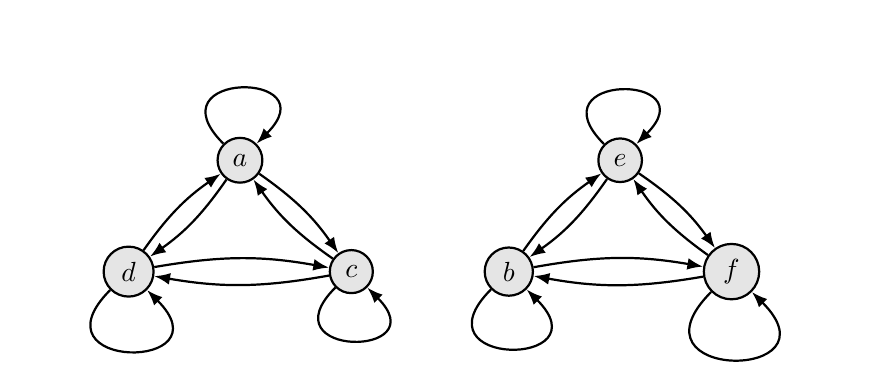
\begin{tikzpicture}[-{Latex[length=2mm]}]
	\node (d) {$d$};
	\node (a) [above right of=d] {$a$};
	\node (c) [below right of=a] {$c$};
	\node (b) [right of=c] {$b$};
	\node (e) [above right of=b] {$e$};
	\node (f) [below right of=e] {$f$};
	\draw (a) to [bend left=10] (c);
	\draw (a) to [bend left=10] (d);
	\draw (d) to [bend left=10] (a);
	\draw (c) to [bend left=10] (a);
	\draw (c) to [bend left=10] (d);
	\draw (d) to [bend left=10] (c);
	\draw (b) to [bend left=10] (f);
	\draw (f) to [bend left=10] (b);
	\draw (a) to [out=135,in=45,looseness=8] (a);
	\draw (c) to [out=225,in=315,looseness=8] (c);
	\draw (d) to [out=225,in=315,looseness=8] (d);
	\draw (e) to [out=135,in=45,looseness=8] (e);
	\draw (b) to [out=225,in=315,looseness=8] (b);
	\draw (b) to [bend left=10] (e);
	\draw (e) to [bend left=10] (f);
	\draw (f) to [bend left=10] (e);
	\draw (e) to [bend left=10] (b);
	\draw (f) to [out=225,in=315,looseness=8] (f);
\end{tikzpicture}

\end{document}

